\documentclass{article}
\usepackage[utf8]{inputenc}
\usepackage[english, russian]{babel}
\usepackage{graphicx}
\graphicspath{ {./graphics/} }
\usepackage[a4paper, total={6in, 8in}]{geometry}
\pagestyle{empty} %
\usepackage[pageanchor]{hyperref}
\usepackage{enumitem}
\usepackage{listings}
\usepackage{amssymb}
\usepackage{amsmath}
\usepackage{indentfirst}
\usepackage{tikz}

\newcommand{\kaucher}{
  \begin{tikzpicture}
    \draw (0, 0) circle (0.6ex);
    \draw (-0.6ex, 0) -- (0.6ex, 0);
  \end{tikzpicture}%
}

\begin{document}
  \begin{titlepage}
    \begin{center}
      Санкт-Петербургский политехнический университет \\Петра Великого
    \end{center}

    \begin{center}
      Физико-механический институт
    \end{center}

    \begin{center}
      Высшая школа прикладной математики и вычислительной\\ физики
    \end{center}

    \vspace{8em}

    \begin{center}
      \textbf{Отчет по лабораторной работе №4}\\
      \textbf{“Интервальный анализ”}
    \end{center}

    \vspace{\fill}

    \begin{flushright}
      \noindentВыполнили студент группы 5030102/10201:
      \hfill
      Скворцов Владимир Сергеевич \\
    \end{flushright}
    Преподаватель: \hfill Баженов Александр Николаевич

    \vspace{12em}

    \begin{center}
      Санкт-Петербург\\
      2024
    \end{center}
  \end{titlepage}

  \tableofcontents

  \newpage

  \section{Постановка задачи}

  Определить параметры линейной регрессии

  \begin{equation} \label{eq:islau}
    \mathbf{y} = \beta_0 + \beta_1 \mathbf{x},
  \end{equation}

  где \( \mathbf{x} \) --- входные данные, \( \mathbf{y} \) --- интервальные
  выходные данные, \( \beta_0 \), \( \beta_1 \) --- параметры линейной
  регрессии.

  Для калибровки измерителя, на вход подаётся набор постоянных
  напряжений

  \begin{equation}
    X = \{ x_i \}.
  \end{equation}

  Для надёжности, для каждого значения \( x \) проводится 100 измерений.

  Получается набор интервальных выборок

  \begin{equation}
    \mathbf{Y} = \{ \mathbf{y}_k \}_{k=1}^{100}.
  \end{equation}

  \( \text{rad} \mathbf{y} = \frac{1}{2^N} \) В, \( N = 14 \).

  Связь кодов данных и В:

  \begin{equation}
    V = \text{Code} / 16384 - 0.5.
  \end{equation}

  Сделать оценки значений \( \mathbf{Y} \) двумя способами:

  \begin{itemize}
    \item in: как интервал между первым и третьим квартилем
    \item ex: как границы бокс-плота
  \end{itemize}

  Решить ИСЛАУ \ref{eq:islau} для внутренних и внешних оценок
  \( \mathbf{y} \)
  Построить множество решений \( \beta_0 \), \( \beta_1 \).
  Построить коридор совместных зависимостей.

  \section{Необходимая теория}

  \subsection{Интервальная мода}

  Пусть имеется интервальная выборка

  \[
    \mathbf{X} = \{ \mathbf{x}_i \}.
  \]

  Сформируем массив интервалов \( \mathbf{z} \) из концов интервалов
  \( \mathbf{X} \).

  Для каждого интервала \( \mathbf{z}_i \) подсчитываем число \( \mu_i \)
  интервалов из выборки \( \mathbf{X}_i \), включающих \( \mathbf{z}_i \).
  Максимальные \( \mu_i = \max \mu \) достигаются для индексного множества
  \( K \). Тогда можно найти интервальную моду как мультиинтервал

  \begin{equation}
    \text{mode} \mathbf{X} = \bigcup_{k \in K} \mathbf{z}_k.
  \end{equation}

  \section{Реализаця}

  Лабораторная работа выполнена на языке программирования Python. В ходе
  работы были также использованы библиотеки \verb!numpy! и
  \verb!matplotlib!.

  Ссылка на GitHub репозиторий:
  \href{https://github.com/vladimir-skvortsov/spbstu-interval-anylysis}
  {https://github.com/vladimir-skvortsov/spbstu-interval-anylysis}

  \subsection{Алгоритм поиска оценок параметров линейной регрессии}

  Каждый из файлов содержит 100 фреймов, каждый из которых включает
  1024 массива, состоящих из 8 двухбайтовых значений. В результате
  обработки этих данных было сформировано \( 1024 \times 8 = 8192 \)
  интервальных систем линейных алгебраических уравнений (ИСЛАУ),
  представленных в следующем виде:

  \[
    \begin{pmatrix}
    [x_1 - \text{rad} \mathbf{y}, x_1 + \text{rad} \mathbf{y}] &
    [1 - \text{rad} \mathbf{y}, 1 + \text{rad} \mathbf{y}] \\
    \vdots & \vdots \\
    [x_8 - \text{rad} \mathbf{y}, x_8 + \text{rad} \mathbf{y}] &
    [1 - \text{rad} \mathbf{y}, 1 + \text{rad} \mathbf{y}]
    \end{pmatrix}
    \begin{pmatrix}
    \beta_1 \\
    \beta_0
    \end{pmatrix}
    = \begin{pmatrix}
    \hat{\mathbf{y}}_{1i} \\
    \vdots \\
    \hat{\mathbf{y}}_{8i}
    \end{pmatrix}, \ i \in \overline{1,8192}
  \]

  Для каждого отдельного пикселя фрейма \( x_j \) обозначает вольтаж,
  определяемый по названию файла, \( \hat{\mathbf{y}}_{ji} \) --- оценка
  значения, соответствующее каждому пикселю, по всем 100 фреймам,
  \( j \) --- порядковый номер файла, а \( i \) --- номер пикселя внутри
  файла. Параметры \( \beta_0 \) и \( \beta_1 \) представляют собой искомые
  параметры линейной регрессии.

  Каждая система линейных алгебраических уравнений была решена с
  использованием метода Дж. Рона \cite{rohn}. В результате были получены
  два множества интервалов оценок:
  \( \mathbf{B}_0 = \{ \mathbf{\beta}_0 \}_{i=1}^{8192} \)
  и \( \mathbf{B}_1 = \{ \mathbf{\beta}_1 \}_{i=1}^{8192} \). Оценка каждого
  из параметров линейной регрессии производится следующим образом:

  \[ \hat{\mathbf{\beta}}_0 = \text{mode} \mathbf{B}_0, \]
  \[ \hat{\mathbf{\beta}}_1 = \text{mode} \mathbf{B}_1. \]

  Таким образом, конечные значения \( \hat{\mathbf{\beta}}_0 \) и
  \( \hat{\mathbf{\beta}}_1 \) служат наиболее вероятными оценками
  параметров регрессии, что позволяет более точно анализировать
  зависимость между переменными в исследуемых данных.

  \section{Результаты}

  \subsection{Внутренняя оценка}

  Для внутренней оценки были получены следующие результаты:

  \[
    \text{mode} \mathbf{B}_0
      = \{ [8086.35, 8086.42], [8086.42, 8086.43], [8086.46, 8086.47], [8086.88, 8086.88] \},
  \]
  \[
    \text{mode} \mathbf{B}_1 = [13070.5, 13072.5].
  \]

  \begin{figure}[htbp!]
		\begin{center}
			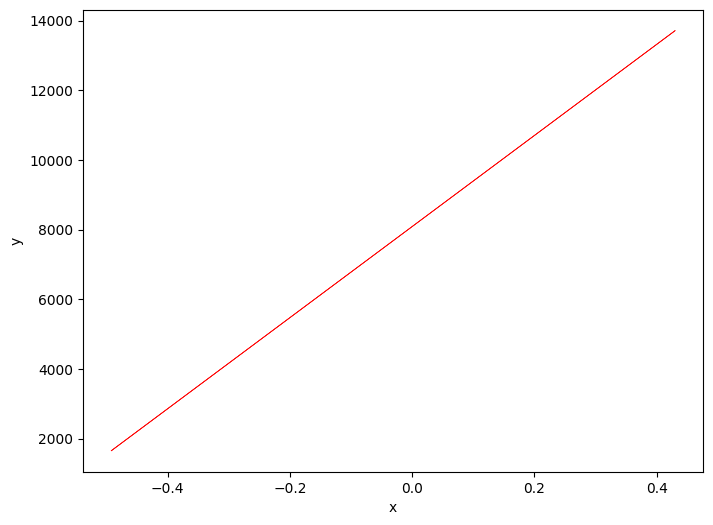
\includegraphics[width = 0.75\textwidth]{int_est}
			\caption{Коридор совместных зависимостей для внутренней оценки.}
      \label{figure:int_est}
		\end{center}
	\end{figure}

  \subsection{Внешняя оценка}

  Для внешней оценки были получены следующие результаты:

  \[
    \text{mode} \mathbf{B}_0 = \bigcap_{i=1}^{8192} \mathbf{\beta}_{0i}
      = [7927.51, 8224.58],
  \]
  \[
    \text{mode} \mathbf{B}_1 = \bigcap_{i=1}^{8192} \mathbf{\beta}_{1i}
      = [13097.9, 13573.8].
  \]

  \begin{figure}[htbp!]
		\begin{center}
			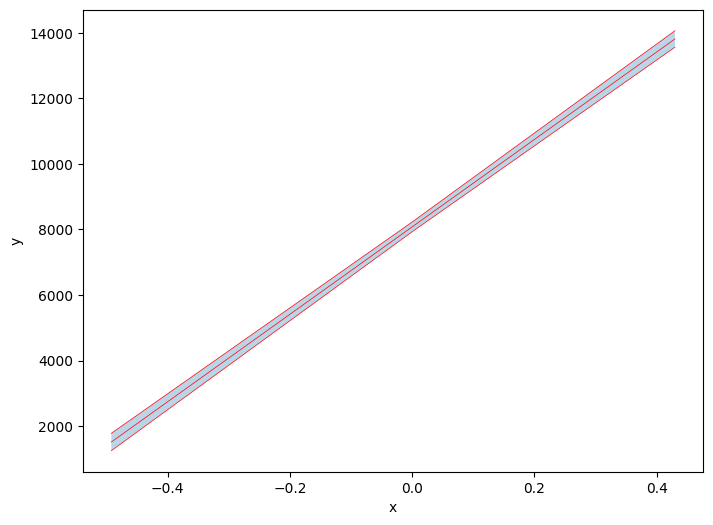
\includegraphics[width = 0.75\textwidth]{ext_est}
			\caption{Коридор совместных зависимостей для внешней оценки.}
      \label{figure:ext_est}
		\end{center}
	\end{figure}

  \section{Вывод}

  В ходе выполнения лабораторной работы была реализована методика оценки
  параметров линейной регрессии на основе интервальных данных. Основные
  результаты включают в себя:

  \begin{itemize}
    \item Разработан алгоритм для нахождения внутренних и внешних оценок
      параметров линейной регрессии, что позволяет учитывать
      неопределённость в данных.
    \item Получены интервальные оценки параметров \( \beta_0 \) и
      \( \beta_1 \), которые демонстрируют диапазон возможных значений
      параметров регрессии.
    \item Построены коридоры совместных зависимостей, которые
      визуализируют интервальные решения и помогают в анализе устойчивости
      модели.
  \end{itemize}

  Результаты показывают, что предложенный подход позволяет более точно
  моделировать зависимости в данных, учитывая возможные вариации и ошибки.
  Это особенно полезно в приложениях, где точность измерений может
  варьироваться, и требуется надёжная оценка параметров модели.

  \bibliographystyle{plain}
  \bibliography{references}

  % TODO: Update the bibliography with relevant references.
  \begin{thebibliography}{9}
    \bibitem{rohn} J. Rohn --- <<Enclosing solutions of overdetermined systems of linear interval equations>>, Reliable Computing 2 (1996), 167-171.
  \end{thebibliography}

\end{document}
